\section{Beschreibung der Anwendung}
\label{sec:beschreibung}
\subsection{Admindialog}
\paragraph{Wohngruppe}\mbox{}\\
Im \textit{Admindialog} können Administratoren Bewohner, Wohngruppen und Mitarbeiter verwalten.
\begin{figure*}[h]
	\begin{center}
		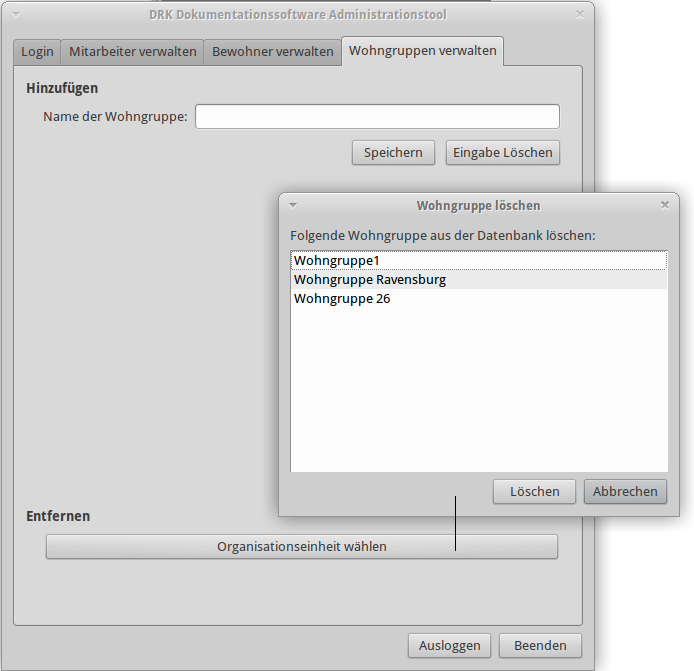
\includegraphics[keepaspectratio=true, width=0.85\textwidth]{pics/admin3.png}
		\caption{Wohngruppe}
		\label{Admindialog Wohngruppe}
		\caption{Graphen eines Interfaces}
		\label{Admindialog_Mitarbeiter_erstellen}
	\end{center}
\end{figure*}
\FloatBarrier
\noindent
Hier werden Wohngruppen erstellt, diese dienen als Gruppierung für sowohl Bewohner, als auch für Mitarbeiter.
\newpage
\noindent
\paragraph{Bewohner}\mbox{}\\
Bewohner werden mit einer Bewohnernummer, Vor-/Nachnamen und ihrer Wohngruppe  erstellt. 
\begin{figure*}[h]
	\begin{center}
		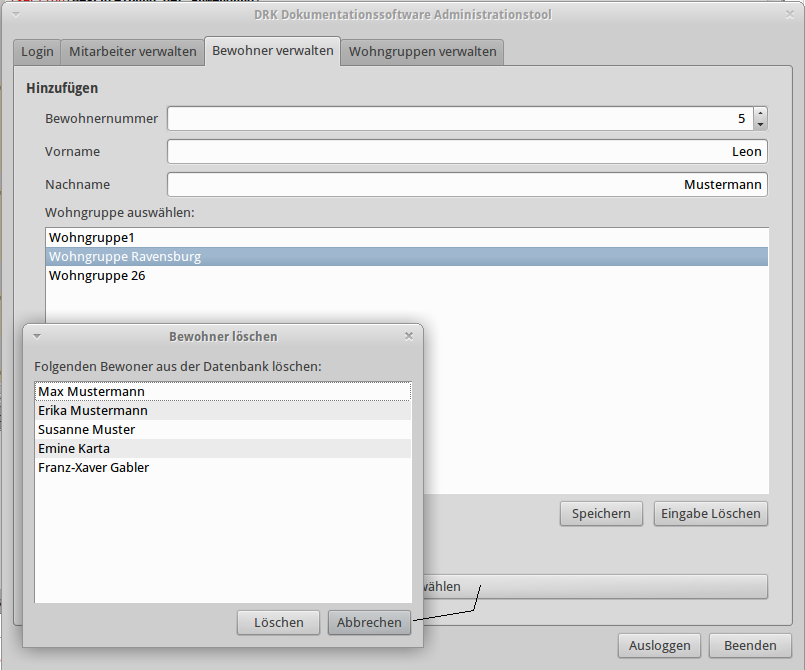
\includegraphics[keepaspectratio=true, width=0.85\textwidth]{pics/admin2.png}
		\caption{Bewohner}
		\label{Admindialog Bewohner}
		\caption{Graphen eines Interfaces}
		\label{Admindialog_Bewohner}
	\end{center}
\end{figure*}
\FloatBarrier
\noindent
Die restlichen Informationen werden im Client von den zuständigen Bezugsbetreuern ausgefüllt.
\newpage
\noindent
\paragraph{Mitarbeiter}\mbox{}\\
Mitarbeiter werden mit einem eindeutigen Login Namen sowie einigen persönlichen Daten, wie Name und Kontaktmöglichkeiten, sowie ihrer Berechtigung
erstellt. Es ist darauf zu achten, dass jedem Mitarbeiter beim Erstellen mindestens eine Wohngruppe zugeordnet werden muss. Mitarbeiter können nur
Informationen von Wohngruppen einsehen, wenn sie diesen Wohngruppen zugeordnet sind. Ein Mitarbeiter kann allerdings auch für mehrere
Wohngruppen zuständig sein und auch der Bezugsbetreuer mehrerer Bewohner sein.
\begin{figure*}[h]
	\begin{center}
		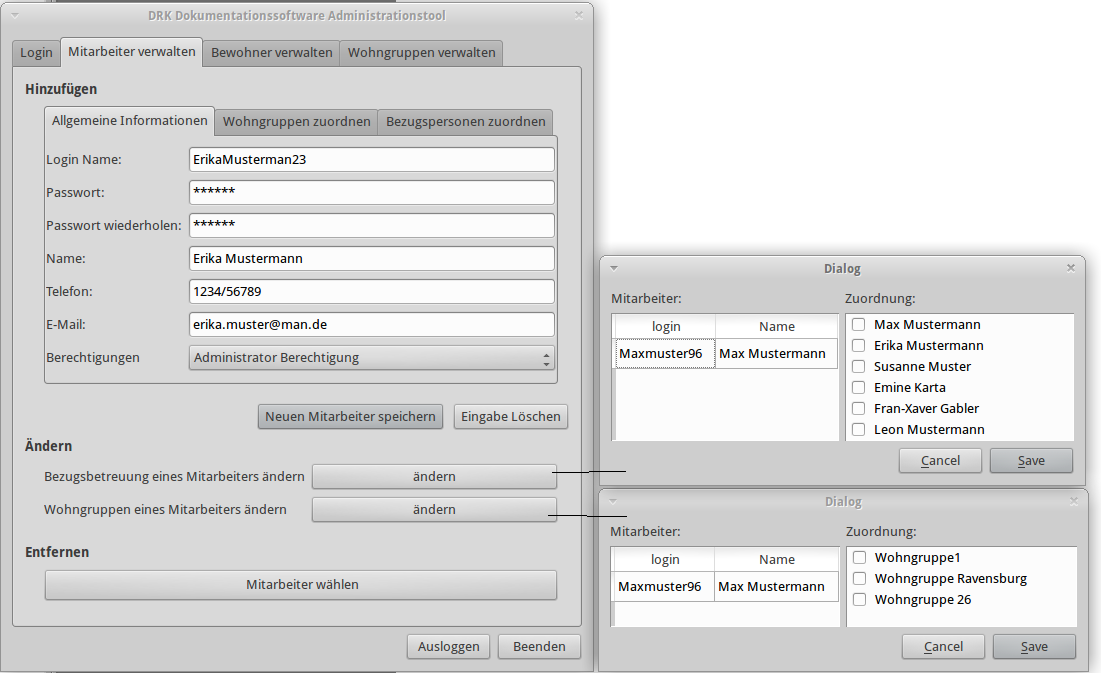
\includegraphics[keepaspectratio=true, width=0.85\textwidth]{pics/admin1.png}
		\caption{Mitarbeiter}
		\label{Admindialog Mitarbeiter}
	\end{center}
\end{figure*}
\FloatBarrier
\noindent
Mitarbeiter die keine Administratorenrechte haben können nur Informationen von Bewohner in ihrer Wohngruppe einsehen. Ändern können sie nur Daten von
Bewohner, deren Bezugsbetreuer sie sind.
\newpage
\subsection{\EBP Client}
Der \EBP \textit{Client} besitzt eine widgetbasierende GUI die aus folgenden Elementen besteht:
\begin{itemize}
	\item Menüleiste\mbox{}\\
	\noindent
	Hier wird der Inhalt des Hauptfensters gespeichert, die zusätzlichen Widgets aus-, bzw eingeblendet oder der Mitarbeiter ausgeloggt.\\ Der
Speichern Button ist ausgegraut, wenn der eingeloggte Mitarbeiter kein Bezugsbetreuer des aktive Bewohners ist.
	\begin{figure*}[h]
		\begin{center}
			
\includegraphics[keepaspectratio=true, width=0.55\textwidth]{pics/client_header.png}
			\caption{Menueleiste}
			%\label{Menüleiste, fixiert an der oberen Seite des Programms}
		\end{center}
	\end{figure*}
	\FloatBarrier
	\noindent
	\item Informationswidget\mbox{}\\
	Hier wird der momentan ausgewählte Bewohner und dessen Wohngruppe angezeigt, zum Ändern öffnet sich, bei Auswahl des jeweiligen Buttons, ein
Popup mit allen Wohngruppen für die der Mitarbeiter berechtigt ist, bzw. alle Bewohner der jeweiligen Wohngruppe.
	\begin{figure*}[h]
		\begin{center}
			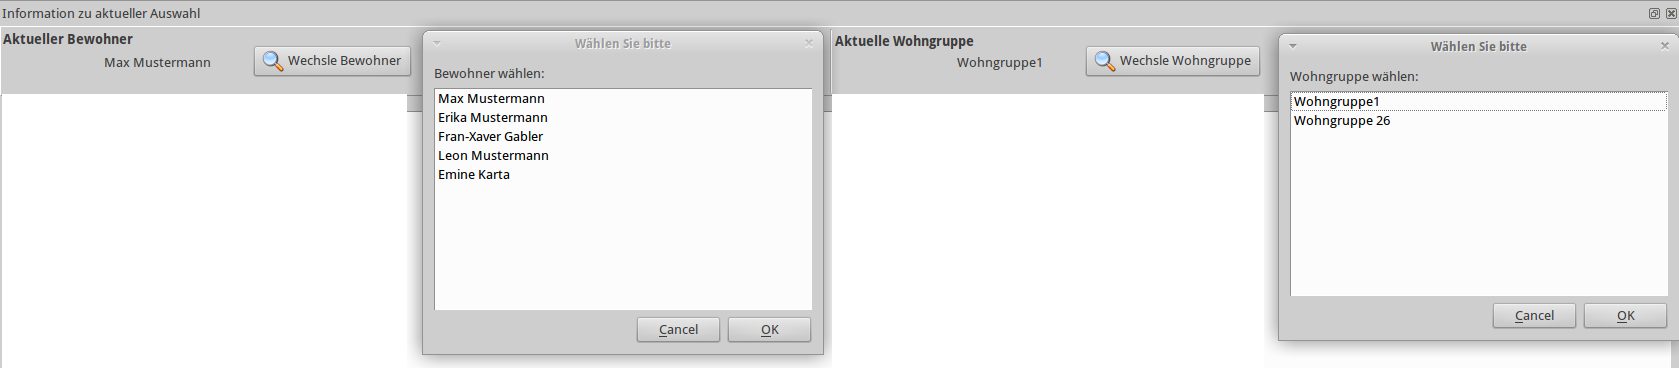
\includegraphics[keepaspectratio=true, width=0.85\textwidth]{pics/client_info.png}
			\caption{Informationswidget}
			%\label{Bewohner- und Stationswidget}
		\end{center}
	\end{figure*}
	\FloatBarrier
	\newpage
	\item Navigationswidget\mbox{}\\
	\noindent
	Im Navigationsmenü wird der Inhalt des Hauptfensters ausgewählt. Das ``Bewohner'' Tab enthält alle Daten und Menüs die sich auf den aktiven
Bewohner beziehen, während das ``Wohngruppen'' Tab Unterpunkte beinhaltet die für die komplette aktuelle Wohngruppe gültig sind.	
	\begin{figure*}[h]
		\begin{center}
			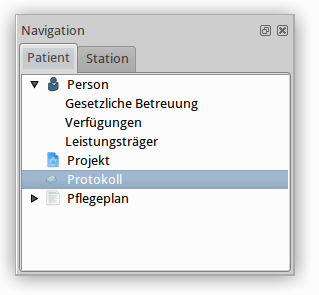
\includegraphics[keepaspectratio=true, width=0.35\textwidth]{pics/client_navi.png}
			\caption{Navigationswidget}
			%\label{Navigationsmenü}
		\end{center}
	\end{figure*}
	\FloatBarrier
	\item Hauptfenster\mbox{}\\
	\noindent
	Das eigentliche Hauptfenster dient zur Ein-/Ausgabe von Daten und bezieht sich immer auf den im Informationswidget ausgewählten Bewohner, bzw die ausgewählte Wohngruppe. Um hier eingegebene Daten zu sichern muss der Speichern-Knopf in der Menüleiste betätigt werden.\\
	\begin{figure*}[h]
		\begin{center}
			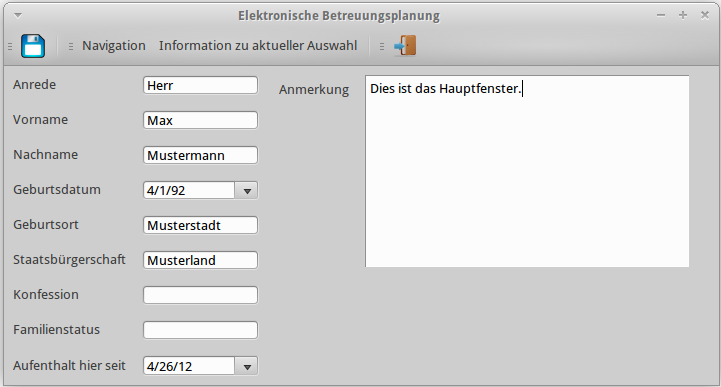
\includegraphics[keepaspectratio=true, width=0.85\textwidth]{pics/client_main.png}
			\caption{Hauptfenster}
			%\label{Hauptfenster}
		\end{center}
	\end{figure*}
	\FloatBarrier
	\newpage
	\item Texttransfer-Interface\mbox{}\\
	\noindent
	Dieses Interface, das in mehreren Menüpunkten am unterem Rand des Hautfensters integriert ist, ermöglicht ein einfaches kopieren von
markierten Textteilen in die Betreungsplanung eines, durch ein Dropdown-Menü auswählbaren, Bewohners.
	\begin{figure*}[h]
		\begin{center}
			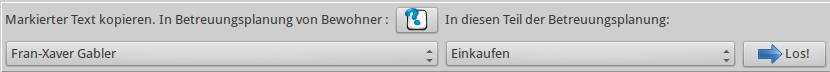
\includegraphics[keepaspectratio=true, width=0.85\textwidth]{pics/client_texttransfer.png}
			\caption{Texttransfer Interface}
		\end{center}
	\end{figure*}
	\FloatBarrier
\end{itemize}
\newpage
\subsubsection{Bewohnerbezogene Masken}
\begin{itemize}
	\item Person\mbox{}\\
	\noindent
	Hier können persönliche Daten des Bewohners eingesehen und geändert werden.
	\begin{figure*}[h]
		\begin{center}
			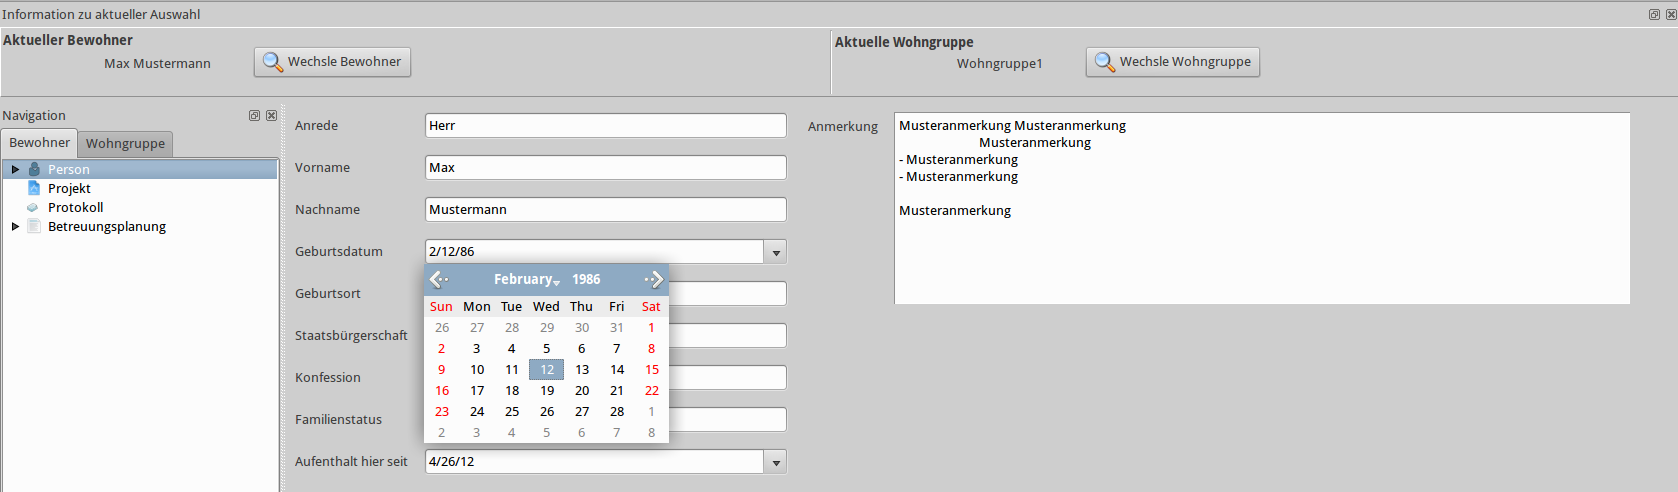
\includegraphics[keepaspectratio=true, width=0.85\textwidth]{pics/client_person.png}
			\caption{Person}
			%\label{Hauptfenster}
		\end{center}
	\end{figure*}
	\FloatBarrier
	\item Gesetzliche Betreuung\mbox{}\\
	\noindent
	Ein Unterpunkt von 'Person'. Hier sind Angaben über den gesetzlichen Betreuer des Bewohners gespeichert.
	\begin{figure*}[h]
		\begin{center}
			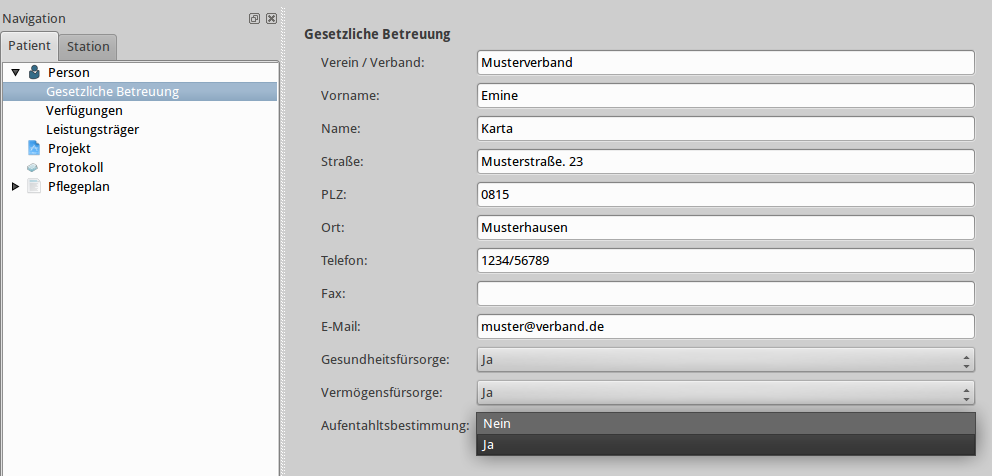
\includegraphics[keepaspectratio=true, width=0.85\textwidth]{pics/client_betreuung.png}
			\caption{Gesetzliche Betreuung}
			%\label{Hauptfenster}
		\end{center}
	\end{figure*}
	\FloatBarrier
	\newpage
	\item Verfügungen\mbox{}\\
	\noindent
	Ein Unterpunkt von 'Person'. Eventuelle Verfügungen, die den Bewohner betreffen, ihre Dauer und Begründung sind hier dokumentiert.
	\begin{figure*}[h!]
		\begin{center}
			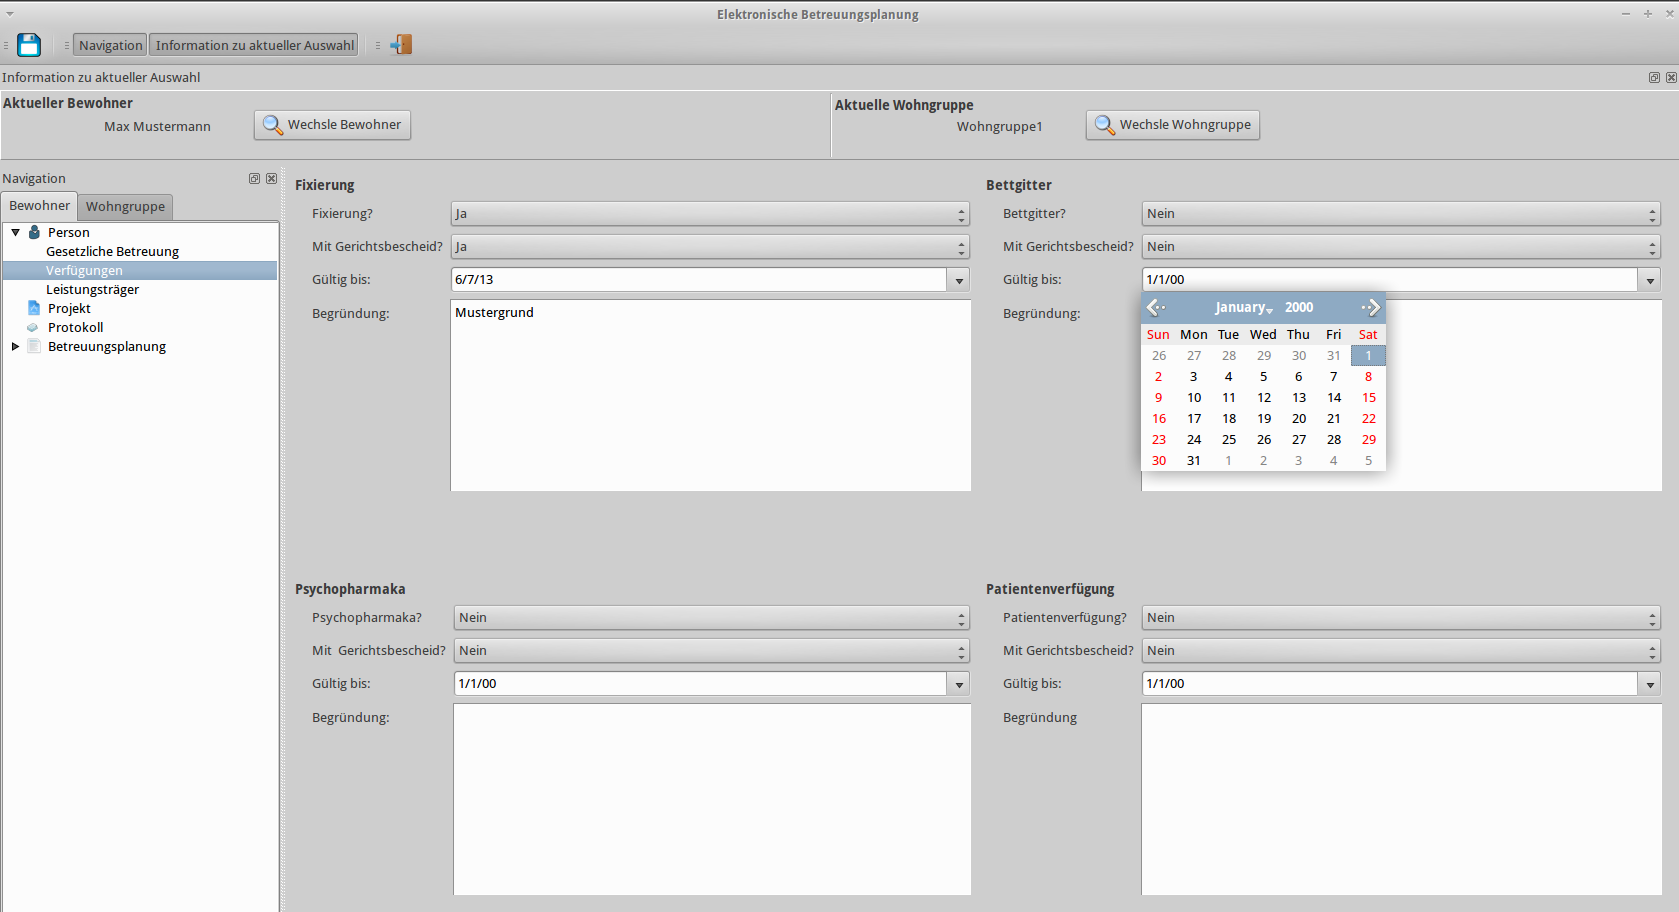
\includegraphics[keepaspectratio=true, width=0.85\textwidth]{pics/client_verfuegung.png}
			\caption{Verfügungen}
			%\label{Hauptfenster}
		\end{center}
	\end{figure*}
	\FloatBarrier
	\item Leistungsträger\mbox{}\\
	\noindent
	Ein Unterpunkt von 'Person'. Durch den Button in der linken, oberen Ecke können Angabemasken für weitere Leistungsträger hinzugefügt werden.
Diese beinhalten sowohl den Leistungsträger an sich, als auch Kontaktdaten eines Ansprechpartners.
	\begin{figure*}[h!]
		\begin{center}
			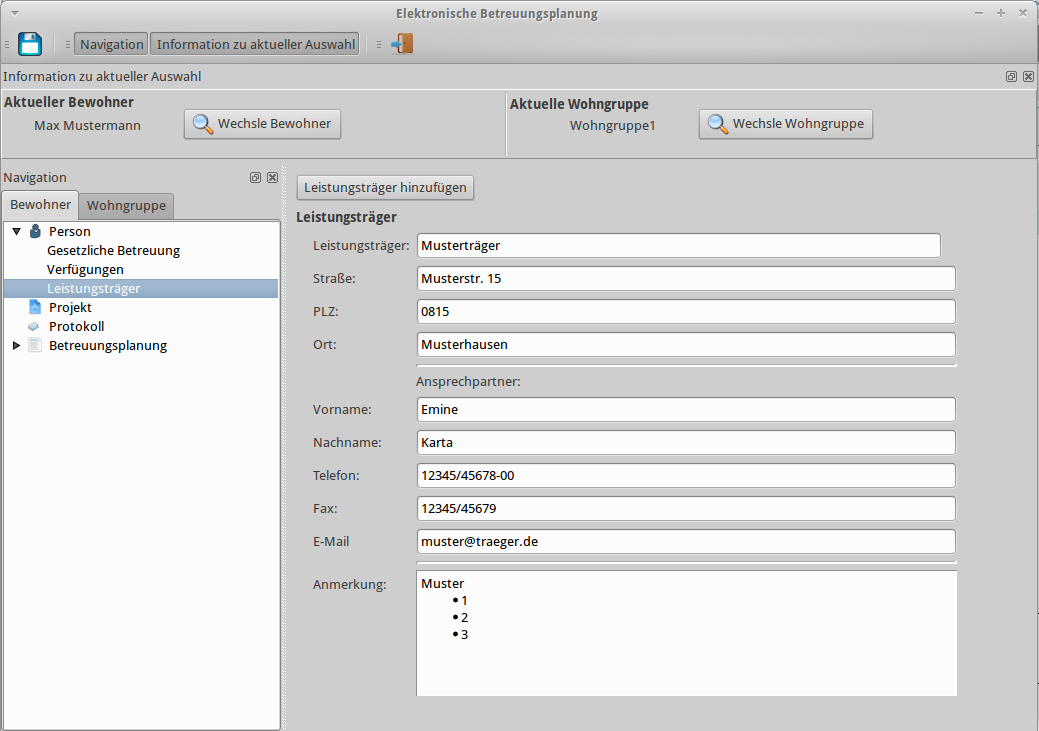
\includegraphics[keepaspectratio=true, width=0.85\textwidth]{pics/client_leistungstraeger.png}
			\caption{Leistungsträger}
			%\label{Hauptfenster}
		\end{center}
	\end{figure*}
	\FloatBarrier
	\newpage
	\item Projekt\mbox{}\\
	\noindent
	Hier werden Projekte mit Zielen, den betreuenden Mitarbeitern und einer Beschreibung für den Bewohner angelegt.\\Am unterem Rand ist eine
Möglichkeit zum einfachem kopieren von ausgewählten Textteilen in die Betreuungsplanung eines auswählbaren Bewohners gegeben.
	\begin{figure*}[h!]
		\begin{center}
			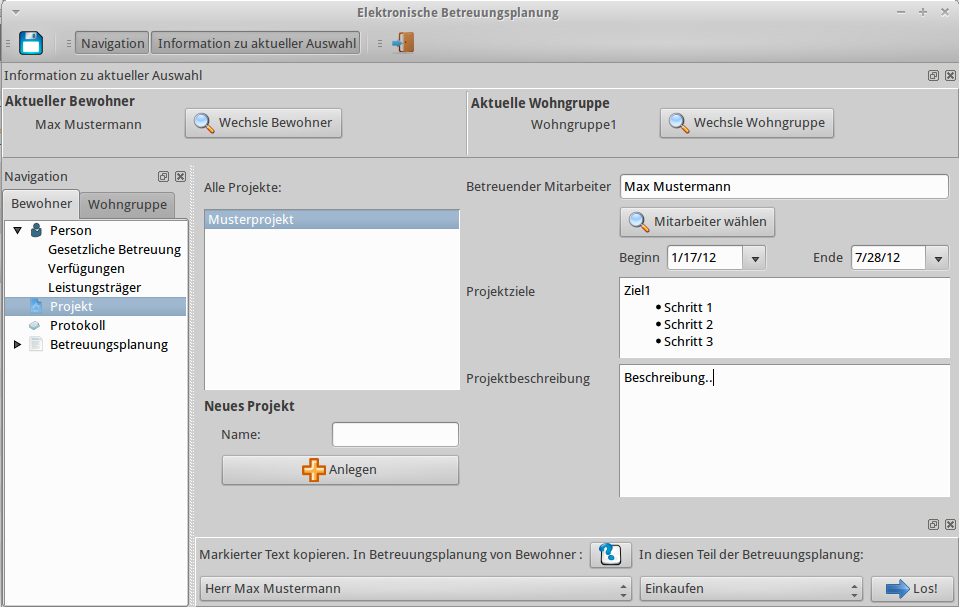
\includegraphics[keepaspectratio=true, width=0.85\textwidth]{pics/client_projekt.png}
			\caption{Projekt}
			%\label{Hauptfenster}
		\end{center}
	\end{figure*}
	\FloatBarrier
	\newpage
	\item Protokoll\mbox{}\\
	\noindent
	Protokolle über Gespräche mit einem Bewohner können hier mit Datum und Uhrzeit erfasst werden. Es kann zudem eine Liste der Teilnehmer
sowie eine Markierung für den Schriftführer angelegt werden.\\Am unterem Rand ist das Texttransfer Interface integriert.
	\begin{figure*}[h!]
		\begin{center}
			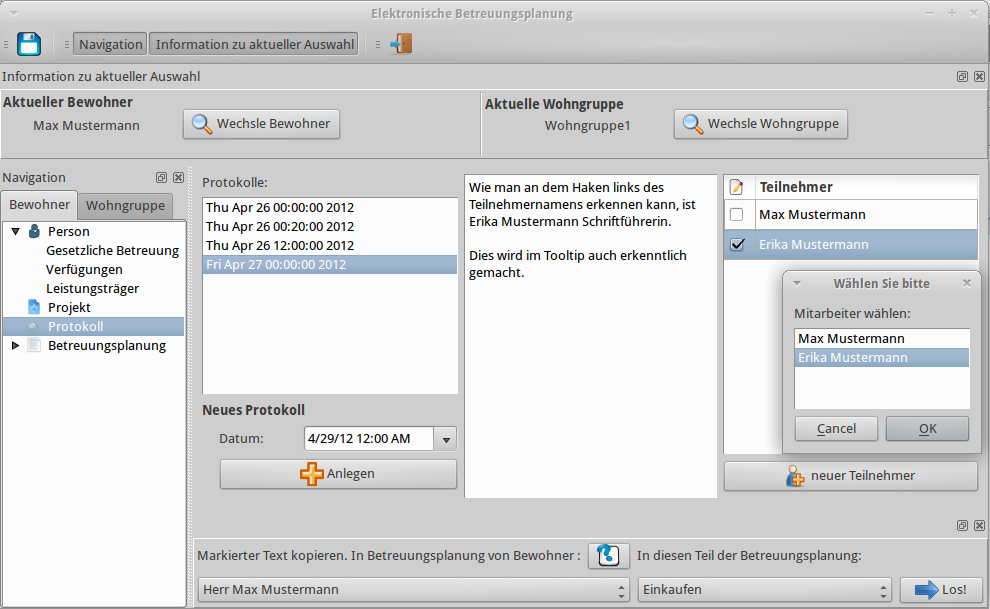
\includegraphics[keepaspectratio=true, width=0.85\textwidth]{pics/client_protokoll.png}
			\caption{Protokoll}
			%\label{Hauptfenster}
		\end{center}
	\end{figure*}
	\FloatBarrier
	\newpage
	\item Betreuungsplanung\mbox{}\\
	\noindent
	in der Betreuungsplanung werden einzelne Fähigkeiten oder Umstände des Bewohners beschrieben, sowohl der momentane Zustand als auch mögliche Ziele die der Bewohner erreichen soll.
	\begin{figure*}[h!]
		\begin{center}
			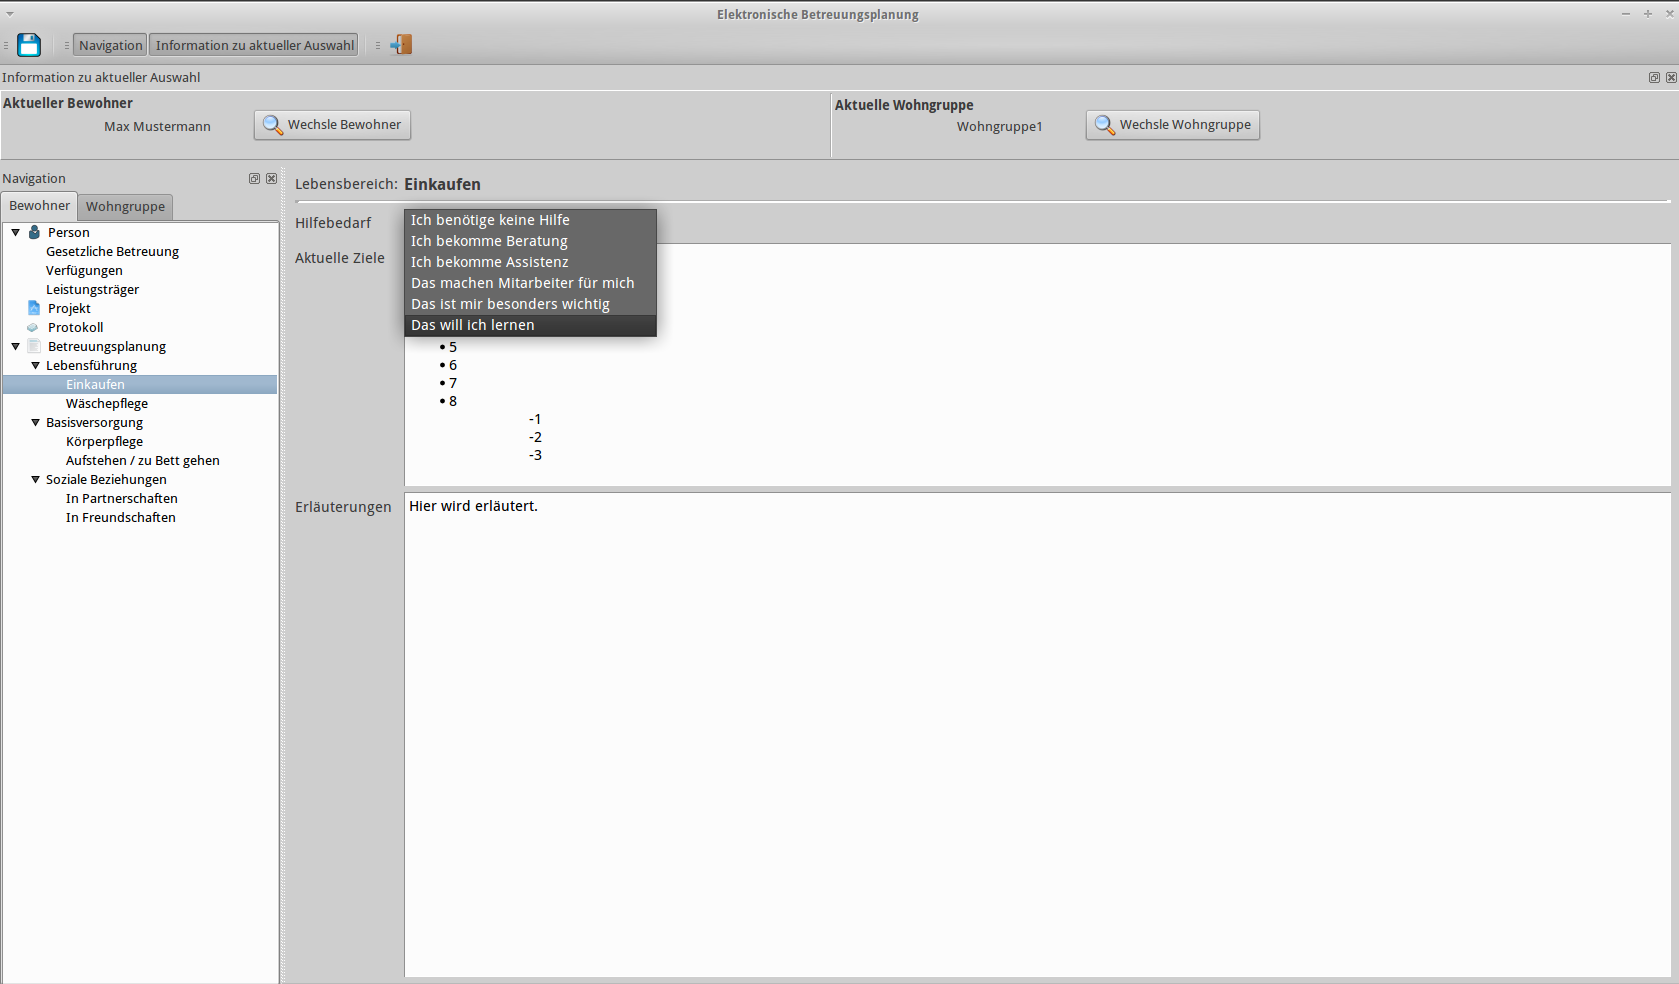
\includegraphics[keepaspectratio=true, width=0.85\textwidth]{pics/client_lebensfuehrung.png}
			\caption{Betreungsplanung: Unterpunkt Einkaufen}
			%\label{Hauptfenster}
		\end{center}
	\end{figure*}
\end{itemize}
\newpage
\subsubsection{Wohngruppen bezogene Masken}
In den Wohngruppen bezogenen Masken können Ereignisse sowie Abwesenheiten sowohl eingetragen, als auch eingesehen werden. Das setzten eines Filters
für einen bestimmten Zeitpunkt ist möglich.
\begin{itemize}
	\item Gruppenbuch\mbox{}\\
	\noindent
	Im Gruppenbuch werden Ereignisse für andere Mitarbeiter protokolliert. Diese Ereignisse bestehen aus einem Datum, den eintragenden Mitarbeiter und einer Beschreibung.\\Standardmäßig werden alle Ereignisse, nach dem Eintragezeitpunkt sortiert, angezeigt. Es ist jedoch möglich die Einträge über einen Zeitbereich zu filtern.\\Am unterem Rand ist das Texttransfer Interface integriert.
	\begin{figure*}[h]
		\begin{center}
			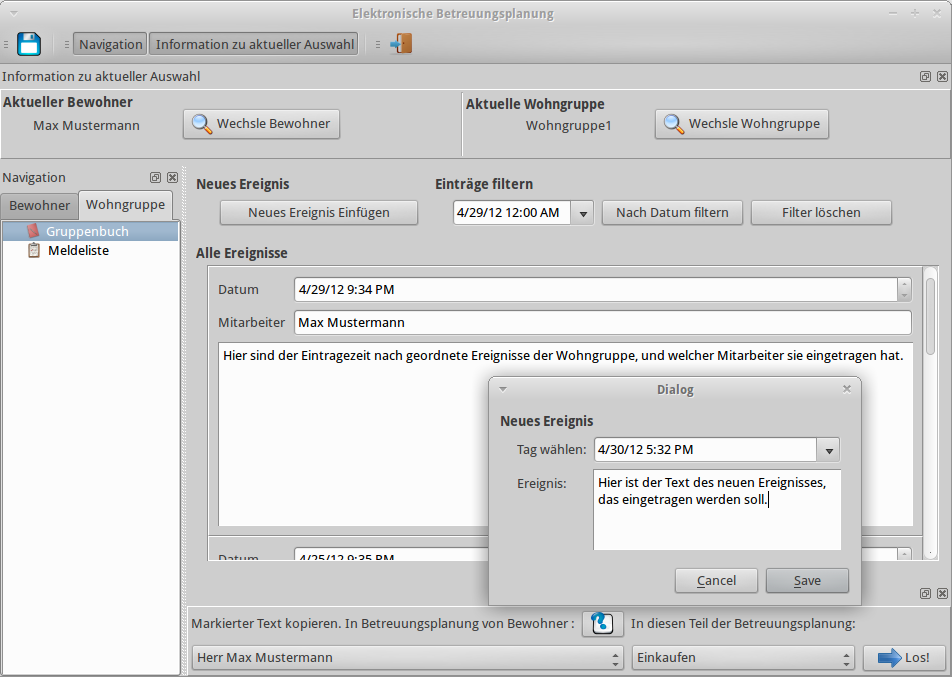
\includegraphics[keepaspectratio=true, width=0.85\textwidth]{pics/client_ereignis.png}
			\caption{Gruppenbuch}
			%\label{Hauptfenster}
		\end{center}
	\end{figure*}
	\FloatBarrier
	\newpage
	\item Meldeliste\mbox{}\\
	\noindent
	In der Meldeliste werden alle Bewohner der Wohngruppe die zu dem ausgewählten Tag bereits in der Wohngruppe anwesend waren angezeigt.
Standardmäßig sind alle Bewohner als 'Anwesend' eingetragen. Es ist nur möglich Bewohner als abwesend zu markieren, wenn ein Grund angegeben wird.\\Es
ist möglich die Abwesenheiten der Bewohner in einem auswählbaren Zeitbereich zu exportieren. Dieser Export ist sowohl im CSV-Format (zur
Weiterverarbeitung in anderen Programmen, z.B. Excel), als auch in Form einer Textdatei mit druckbarer Formatierung möglich.
	\begin{figure*}[h]
		\begin{center}
			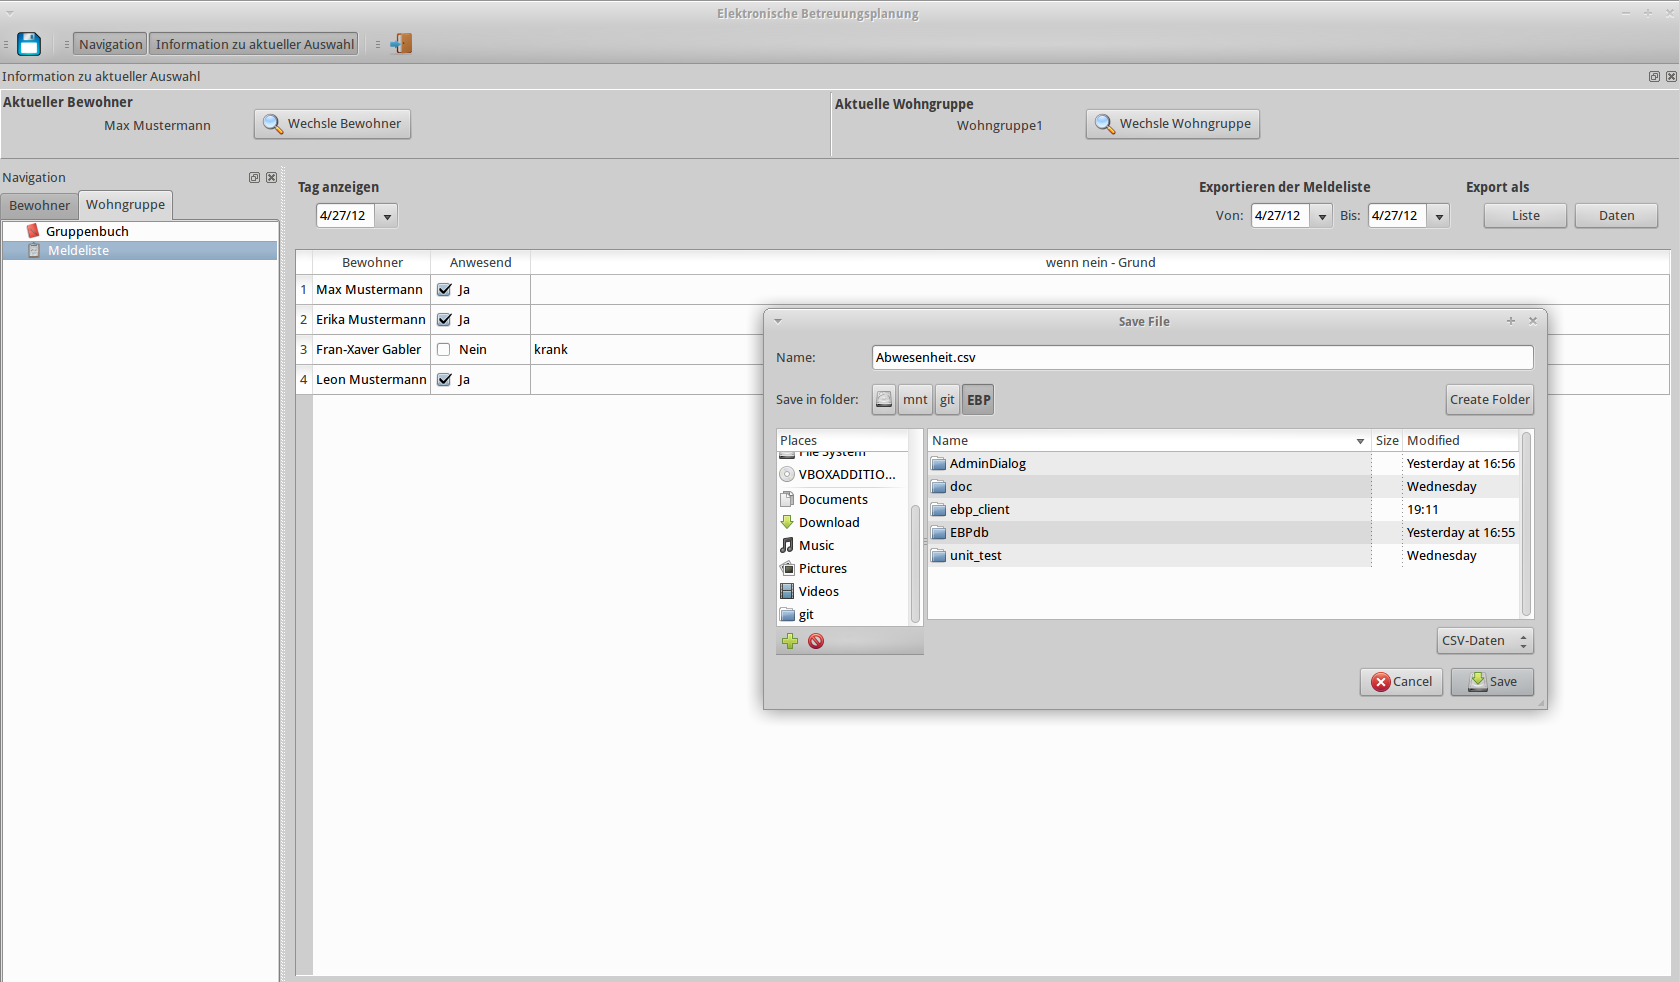
\includegraphics[keepaspectratio=true, width=0.85\textwidth]{pics/client_meldeliste.png}
			\caption{Meldeliste}
			%\label{Hauptfenster}
		\end{center}
	\end{figure*}
	\FloatBarrier
\end{itemize}
\newpage

\subsection{Konfiguration}
Für den \textit{AdminDialog} und die \EBP gibt es die Möglichkeit in einer Konfigurationsdatei (AdminDialog.ini und EBP.ini) die verwendete Datenbank,
den Host der Datenbank und die entsprechende Portnummer festzulegen. Es gilt folgende Notation:
\begin{lstlisting}
[General]
db=ebp_Sozialwerk			//Datenbankname
host=10.10.10.10			//Host der Datenbank
port=8888					//Portnummer	
\end{lstlisting}
Werden in den .ini Dateien keine Werte angegeben gelten folgende Werte implizit als Defaultwerte:
\begin{lstlisting}
db=ebp
host=localhost
port=3306
\end{lstlisting}
\subsection{Lokalisierung}
Sowohl der \textit{AdminDialog} als auch die \EBP sind komplett lokalisierbar. \textit{Qt} stellt dafür einen einfachen Mechanismus zur Verfügung. Jeder zu
lokalisierende String wird dabei von einem Makro umschlossen. Mit Hilfe des \textit{Qt} Linguist können diese Strings zu einem Wörterbuch zusammengefasst und
übersetzt werden. Für die \EBP war im Pflichtenheft angedacht, ein englisches und eine deutsches Wörterbuch zur Verfügung zu stellen. In den
Gesprächen zur Anforderungsdefinition mit Herrn Zimmer zeichnete sich ein anderer Lokalisierungsbedarf an die \EBP ab.\\
Die Fachkräfte in der Altenhilfe und der Behindertenhilfe haben ihre eigene Fachsprache im täglichen Umgang mit ihren Klienten. So liegt der Fokus in
der Altenhilfe eher auf pflegerischen Tätigkeiten, wohingegen in der Behindertenhilfe pädagogische Ziele und Maßnahmen im Vordergrund stehen. Ein
Klient wird in der Altenhilfe eher als Patient bezeichnet, in der Behindertenhilfe spricht man häufiger von einem Bewohner. Um diesen Umstand zu
berücksichtigen, wurden keine Wörterbücher für Englisch und Deutsch erstellt, sondern Wörterbücher für die Altenhilfe und für die Behindertenhilfe.\\
Wird der Client oder der \textit{AdminDialog} ohne Parameter gestartet, wird das Wörterbuch der Behindertenhilfe geladen. Um die Lokalisierung der Altenhilfe
zu aktivieren, muss der entsprechenden Anwendung der Parameter ``-a'' übergeben werden.

\newpage

\subsection{Erstellen der Anwendung}
\subsubsection{Abhängigkeiten}
\paragraph{Zur Laufzeit:}
\begin{itemize}
	\item \textbf{odb} - \textit{ODB} Laufzeitbibliothek
	\item \textbf{odb-mysql} - \textit{MySQL} Backend für \textit{ODB}
	\item \textbf{odb-qt} - \textit{Qt} integration für \textit{ODB}
	\item \textbf{qt} - \textit{Qt} Framework
\end{itemize}
\paragraph{Zur Compilezeit:}
\begin{itemize}
	\item \textbf{CMake} - Buildsystem
	\item \textbf{ODB Toolchain} - Enthält den Precompiler
	\item \textbf{GCC} - \textit{GNU} Compiler Collection
\end{itemize}
\subsubsection{Kompilieren der Quellen}
Die komplette Anwendung kann im Wurzelverzeichnis des Projekts gebaut werden:\\
\begin{lstlisting}
$ cmake .
\end{lstlisting}
Generiert das benötigte Makefile.\\
Ist dies erfolgreich abgeschlossen, wird mit\\
\begin{lstlisting}
$ make
\end{lstlisting}
der eignetliche Kompiliervorgang gestartet.\\
\subsubsection{Vorbereiten der Datenbank}
Um die Datenbank zu initialisieren befindet sich ein Shell-Script im \textit{EBPdb} Verzeichnis:\\
\begin{lstlisting}
$ ./initDB.sh -u root -p "DATENBAKNAME"
\end{lstlisting}
